\documentclass[11pt,a4paper]{article}
\usepackage{gtu-el-yazisi}
\begin{document}
\notbilgi{Elektronik II}{Final çalışması: geri besleme ve frekans cevabı}{Final-notu.pdf}

\sayfa{1}
\section{Feedback}
\subsection{The general feedback structure}

\begin{center}
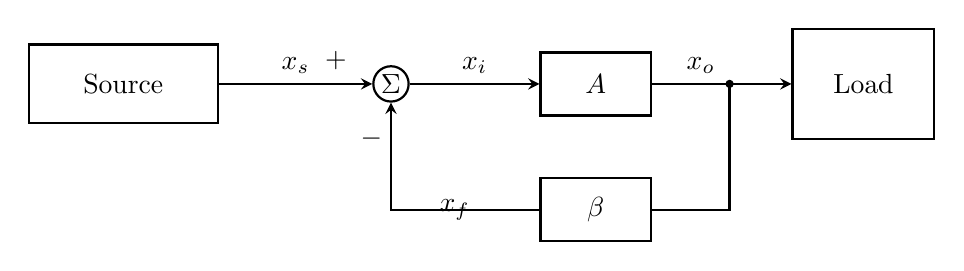
\begin{tikzpicture}[line width=0.8pt,>=stealth]
  \node[draw,minimum width=2.4cm,minimum height=1cm] (src) at (0,0) {Source};
  \node[draw,circle,inner sep=1pt] (sum) at (3.4,0) {$\Sigma$};
  \node[draw,minimum width=1.4cm,minimum height=0.8cm] (A) at (6.0,0) {$A$};
  \node[draw,minimum width=1.8cm,minimum height=1.4cm] (load) at (9.4,0) {Load};
  \node[draw,minimum width=1.4cm,minimum height=0.8cm] (B) at (6.0,-1.6) {$\beta$};
  \draw[->] (src) -- node[above,pos=0.5] {$x_s$} (sum);
  \node at (2.7,0.3) {$+$};
  \draw[->] (sum) -- node[above] {$x_i$} (A);
  \draw[->] (A) -- node[above,pos=0.35] {$x_o$} (load);
  \fill (7.7,0) circle (1.5pt);
  \draw (7.7,0) |- (B.east);
  \draw[->] (B.west) -| node[left,pos=0.2] {$x_f$} (sum.south);
  \node at (3.15,-0.7) {$-$};
\end{tikzpicture}
\end{center}

\noindent
\begin{minipage}[t]{0.42\linewidth}
$A$ = open loop gain\\[1mm]
$\beta$ = feedback factor\\[1mm]
$x_i$ = Input signal\\[1mm]
$x_s$ = signal source\\[1mm]
$x_o$ = output signal\\[1mm]
$x_f$ = sampled output
\end{minipage}\hfill
\begin{minipage}[t]{0.54\linewidth}
\vspace{-3mm}
\begin{align*}
\left(\frac{x_o}{x_s}\right)_{CL} &= \ ? \\
x_o &= A\,x_i \\
x_f &= \beta \cdot x_o \\
x_i &= x_s - x_f \\
x_i &= x_s - \beta\, x_o \\
x_i &= x_s - A\beta\, x_i \\
x_s &= x_i\,(1+A\beta)
\end{align*}
\end{minipage}

\[ \left(\frac{x_o}{x_s}\right) = \frac{A\,x_i}{x_i\,(1+A\beta)} = \frac{A}{1+A\beta} \]

\sekilnotu[1]{Evirmeyen (non-inverting) op-amp devresi: $A$ kazançlı op-amp; ``$+$'' ucuna toprağa bağlı $v_i$ kaynağı; ``$-$'' ucu $R_1$ ile toprağa ve $R_2$ üzerinden çıkışa (geri besleme) bağlı; çıkış $v_o$.}

\[ \frac{v_o}{v_i} = \left(1+\frac{R_2}{R_1}\right) \approx \frac{1}{\beta} \]
\[ \beta = \left(1+\frac{R_2}{R_1}\right)^{-1} \]

\subsection{Voltage Amplifiers (Shunt-Series)}
\sekilnotu[1]{Gerilim yükselteci (shunt-series) blok diyagramı: $V_s$ kaynağı ve $R_s$ üzerinden ``Basic Amplifier'' kutusunun girişi; kutunun çıkışında $R_L$ yük direnci ve ``$+\ V_o\ -$'' uçları; çıkış düğümünden ``Feedback'' kutusuna paralel bağlantı (kırmızı elips ve kırmızı ``Shunt'' notu); ``Feedback'' kutusunun çıkışı ($V_f$, ``$+$'' üstte, ``$-$'' altta) giriş döngüsüne seri bağlı (kırmızı ``Series'' notu ve ok). Turuncu kalemle $R_{if}$, $R_{in}$, $R_{out}$ ve $R_{of}$ okları işaretlenmiş.}

\subsection{Two port network equivalent}
\sekilnotu[1]{İki kapılı eşdeğer devre: $V_s$ kaynağı (``$+$'' üstte), üst kolda $R_s$, alt kolda $R_{11}$ ve ``Basic Amplifier'' kutusu; çıkışta paralel $R_{22}$ ve $R_L$, $v_o$ (``$+$'' üstte, ``$-$'' altta). Solda $R_i$ oku, sağda $R_o$ oku. Kırmızı bir ok çıkıştaki dirençleri ``feed forward gain $A = v_o/v_s$'' notuna bağlıyor.}

\sekilnotu[1]{Geri besleme ağı iki kapılısı (``feedback'' kutusu): sol çizim: sol kapı iki açık uç (``$\pm$'' işaretli, yanında ok ve ``$R_{11}$''), sağ kapının uçları birbirine kısa devre. Sağ çizim: ``feedback'' kutusunun sol uçları açık, sağ kapıda ok ile ``$R_{22}$''. Altta ``To find $\beta$'': sol kapıdan $I_1$ akımı (ok) ve $V_f$ (``$+$'' üstte, ``$-$'' altta); sağ kapıya $V_o$ kaynağı bağlı.}

\formulkutu{\beta = \frac{V_f}{V_o}\Big|_{I_1}}

\sayfa{2}
\subsection{Complete model}
\sekilnotu[2]{Gerilim geri beslemeli yükseltecin tam modeli: $v_s$ kaynağı (``$+$'' üstte), $R_s$ ve $R_i$ (üzerinde $v_i$, ``$+$'' üstte) giriş çevrimi; çıkışta $R_o$ ile seri bağımlı gerilim kaynağı $A v_i$ ve çıkış uçları ``$+\ v_o\ -$''; giriş çevrimine seri, alt kolda bağımlı gerilim kaynağı $\beta V_o$ ve yanında $v_o$ (``$+$'' üstte, ``$-$'' altta). Turuncu kesikli çerçeveler: ``A circuit'' ve ``$\beta$ circuit''; turuncu notlar: $R_{if}$ (S ve S' uçları işaretli) ve $R_{of}$.}

\sekilnotu[2]{Sadeleştirilmiş eşdeğer devreler: solda S--S' uçları (``$v_s$'', ``$+$'' üstte) ve $R_{if}$; sağda bağımlı gerilim kaynağı $A_f v_s$, $v_o$ (``$+$'' üstte) ve $R_{of}$.}

\[ A_f = \frac{A}{1+A\beta} \qquad\qquad R_{if} = (1+A\beta)\,R_i \qquad\qquad R_{of} = \frac{R_o}{(1+A\beta)} \]

\subsection{Current Amplifier feedback}
\sekilnotu[2]{Akım geri beslemeli yükselteç modeli: $I_s$ akım kaynağı (yukarı ok, ``S'' ucu), $I_s$ oku, $R_i$ (üzerinde $V_i$, ``$+$'' üstte); bağımlı akım kaynağı $A I_i$ ve $R_o$; çıkış akımı $I_o$ ve $R_{of}$; geri besleme kolunda bağımlı akım kaynağı $\beta I_o$; S' ucu ve $R_{if}$ oku solda. Turuncu kesikli çerçeve: ``$\beta$ circuit''.}

\sekilnotu[2]{Eşdeğer devreler: solda S ve S' uçları, $I_s$ oku ve $R_{if}$; sağda bağımlı akım kaynağı $A_f I_s$, $R_{of}$ ve $I_o$ akımı.}

\[ A_f = \frac{A}{1+A\beta} \]
\[ R_{if} = \frac{R_i}{1+A\beta} \]
\[ R_{of} = R_o\,(1+A\beta) \]

\sayfa{3}
\section{Soru}
\sekilnotu[3]{Geri besleme ağı örnekleri: iki çizimde de üst hatta seri $R_2$, ve toprağa bağlı paralel $R_1$. Sol çizim: çıkış uçları turuncu çizgiyle kısa devre, sol kapıda turuncu ok ve ``$R_{11}$''. Sağ çizim: çıkış uçları açık, giriş uçları turuncu ``o'' ile işaretli, sağ kapıda turuncu ok ve ``$R_{22}$''.}

\[ R_{11} = R_1 \parallel R_2 \qquad\qquad R_{22} = R_1 + R_2 \]

\sekilnotu[3]{$V_f$ devresi: solda $V_f$ uçları (``$+$'' üstte), toprağa bağlı dikey $R_1$, üst hatta seri $R_2$ ve sağda $V_o$ kaynağı.}

\[ \frac{V_f}{V_o} = \frac{R_1}{R_1+R_2} = \beta \]

\[ R_{eq} = R_s + R_{id} + R_{11} = \]

\sekilnotu[3]{Yükseltecin giriş tarafı: iki açık uç ($v_s$, ``$+$'' üstte, ``$-$'' altta), üst kolda $R_s$, sağda $R_{id}$ (üzerinde $v_1$, ``$+$'' üstte), alt kolda $R_{11}$ (``$R_{11}=??$''); solda $R_i$ oku. Çıkış tarafı: bağımlı gerilim kaynağı $A_0 v_1$, $r_o$, paralel $R_{22}$ ve $R_L$, çıkış $v_o$; $R_o$ oku.}

\[ \frac{v_o}{v_1} = \frac{R_{22} \parallel R_L}{r_o + R_{22} \parallel R_L}\cdot A_0 \]

\[ A = \frac{v_o}{v_s} = \frac{v_o}{v_1}\cdot\frac{v_1}{v_s} \]

\[ \frac{v_1}{v_s} = \frac{R_{id}}{R_s+R_{id}+R_{11}}\cdot\frac{v_s}{v_s} \]
\textit{(sağdaki $v_s/v_s$ çarpanı çizilerek sadeleştirilmiş)}

\[ A = \frac{R_{id}}{\underbrace{R_s+R_{id}+R_{11}}_{R_i}}\cdot\frac{R_{22} \parallel R_L}{r_o + R_{22} \parallel R_L}\cdot A_0 \]

\[ A_f = \frac{A}{1+A\beta} \qquad\qquad \beta = \frac{R_1}{R_1+R_2} \]

\sayfa{4}
\[ R_{if} = (1+A\beta)\,R_i \qquad\qquad R_{of} = \frac{R_o}{(1+A\beta)} \]

\noindent (\okunamadi{O}) \qquad\quad (I)

\subsection{Series -- Series feedback Topology}
\noindent -Suitable for transconductance Amplifier

\sekilnotu[4]{Series-series geri besleme blok diyagramı: $V_s$ kaynağı (``$+$'' üstte), $R_s$ ve ``Basic Transconductance Amplifier'' kutusu; çıkışta $I_o$ oku ve $R_L$ yükü; ``$f_B$'' etiketli geri besleme kutusu çıkış akımını ($I_o$ oku) örnekliyor, çıkışı $V_f$ (``$+$'' üstte) olarak giriş döngüsüne seri bağlı.}

\sekilnotu[4]{Tam model: $V_s$ kaynağı, S ve S' uçları; $R_i$ (üzerinde $v_i$, ``$+$'' üstte), bağımlı akım kaynağı ``$A_o v_i$'' ve $R_o$ (kırmızı kesikli çerçeve: ``A circuit''); giriş döngüsüne seri bağımlı gerilim kaynağı $\beta I_o$ (kırmızı kesikli çerçeve: ``$\beta$ circuit''); çıkış uçları O ve O'.}

\subsection{Two port equivalent circuit}
\sekilnotu[4]{İki kapılı eşdeğer devre: $V_i$ kaynağı (``$+$'' üstte), üst kolda $R_s$, alt kolda $R_{11}$ ve ``BTA'' kutusu; kutunun çıkışında üst hatta $I_o$ oku ve $R_L$, alt hatta $R_{22}$; açık uçlar ve $R_o$ oku. Altında iki ``FN'' (feedback network) çizimi: üstteki çizimde sol kapı açık uçlar ($R_{11}$) ve sağ kapı açık uçlar ($R_{22}$); alttaki çizimde sol kapıda $I_f = 0$ ve $V_f$ (``$+$'' üstte, ``$-$'' altta), sağ kapıya $I_o$ akım kaynağı bağlı.}

\formulkutu{\frac{I_o}{V_1} = A}

\[ \beta = \frac{V_f}{I_o} \]

\[ R_{if} = R_i\,(1+A\beta) \]
\[ R_{of} = R_o\,(1+A\beta) \]
\[ A_f = \frac{A}{1+A\beta} \]

\sayfa{5}
\subsection{Two-port equivalent circuit}
\sekilnotu[5]{Önceki sayfadakine benzer iki kapılı eşdeğer devre: $V_i$ kaynağı (``$+$'' üstte), üst kolda $R_s$, alt kolda $R_{11}$ ve ``BTA'' kutusu; çıkışta $I_o$ oku, $R_L$, $R_{22}$ ve $R_o$ oku. Altında ``FN'' çizimleri: açık uçlu sol kapı ($R_{11}$ oku) ve sağ kapı ($R_{22}$ oku); ikinci ``FN'' çiziminde sol kapıda $I_f = 0$ ve $V_f$ (``$+$'' üstte), sağ kapıda $I_o$ akım kaynağı.}

\formulkutu{\frac{I_o}{V_1} = A}

\[ \beta = \frac{V_f}{I_o} \]

\[ R_{if} = R_i\,(1+A\beta) \]
\[ R_{of} = R_o\,(1+A\beta) \]
\[ A_f = \frac{A}{1+A\beta} \]

\subsection{Shunt -- Shunt feedback topology}
\noindent (Trans resistance amplifier)

\sekilnotu[5]{Shunt-shunt geri besleme blok diyagramı: $I_s$ akım kaynağı ve paralel $R_s$; ``Base TRA'' kutusu; çıkışta $R_L$ ve $v_o$ (``$+$'' üstte); ``FBN'' kutusu: sol tarafta $I_f$ akımı (``$+$'' ve ``$-$'' işaretli uçlar), sağ tarafta $I_o$ ve $v_o$ (``$+$'' solda); FBN girişi yükselteç girişine, çıkışı yükselteç çıkışına paralel bağlı.}

\[ A = \frac{V_o}{I_s} \]

\sekilnotu[5]{Tam model: $I_s$ akım kaynağı (yukarı ok), S ve S' uçları; $R_i$ (üzerinde $V_i$, ``$+$'' üstte), bağımlı gerilim kaynağı ``$A I_i$'' ve $R_o$ (kırmızı kesikli çerçeve: ``A circuit''); çıkış uçları O ve O'; giriş düğümüne bağlı bağımlı akım kaynağı $\beta V_o$ (aşağı ok); sağ altta $V_o$ uçları (``$+$'' üstte, ``$-$'' altta).}

\sayfa{6}
\sekilnotu[6]{Shunt-shunt iki kapılı eşdeğer devre: $I_i$ akım kaynağı (yukarı ok), $R_i$ oku, paralel $R_s$ ve $R_{11}$, ``BTRA'' kutusu, çıkışta paralel $R_{22}$ ve $R_L$, $R_o$ oku ve $V_o$ uçları (``$+$'' üstte, ``$-$'' altta).}

\sekilnotu[6]{Üç ``FN'' çizimi: (sol) giriş uçları açık, $R_{11}$ oku, çıkış uçları kısa devre; (sağ) giriş uçları kısa devre, çıkış uçları açık, $R_{22}$ oku; (alt) giriş tarafında $I_f$ oku (kısa devre), çıkışa $V_o$ kaynağı bağlı.}

\[ \beta = \frac{I_f}{V_o} \]

\[ R_{if} = \frac{R_i}{1+A\beta} \]
\[ R_{of} = \frac{R_o}{1+A\beta} \]
\[ A_f = \frac{A}{1+A\beta} \]

\begin{ornek}[2]
ignore $r_o$ $\parallel$ \qquad $\beta = 100$ \quad $(V_A = \infty)$

\sekilnotu[6]{BJT yükselteç devresi: $12\ \mathrm{V}$ besleme (yukarı ok), $4{,}7\mathrm{k}$ kolektör direnci; kolektör ile base arasında $47\mathrm{k}$ geri besleme direnci; sinüs kaynağı ve ona seri $10\mathrm{k}$ direnç base düğümüne bağlı; base-emiter üzerinde ``$+\ 0{,}7\ -$''; emiter toprakta. Kolektör düğümü kırmızı noktalı ve kırmızı bir çıkış ucuna bağlı; solda $R_{in}$ oku.}
\end{ornek}

\noindent DC

\sekilnotu[6]{DC devresi: $12\ \mathrm{V}$, $4{,}7\mathrm{k}$ (kolektör, $V_C$ düğümü, $I_C$ oku), kolektör--base arası $47\mathrm{k}$ (üzerinde akım oku, etiketi ``$I_9$'' gibi okunuyor), base kolunda toprağa $10\mathrm{k}$ (üzerinde sola ``0,07 mA'' oku), base-emiter ``$0{,}7\mathrm{V}$'' ($+$ solda) ve $I_B$ oku; emiter toprakta.}

\[ \frac{0{,}7}{10\mathrm{k}} = 0{,}07\ \mathrm{mA} \]

\[ \frac{12-V_C}{4{,}7} = I_C + \frac{V_C-0{,}7}{47\mathrm{k}} \]


\sayfa{7}
\[ I_C = \frac{12-V_C}{4{,}7\mathrm{k}} - \frac{V_C-0{,}7}{47\mathrm{k}} \]

\[ I_C = \frac{120-11\,V_C+0{,}7}{47\mathrm{k}} \]

\[ \frac{V_C-0{,}7\ \mathrm{V}}{47\mathrm{k}} = I_B + 0{,}07\ \mathrm{mA} \]

\[ I_B = \frac{V_C-0{,}7}{47\mathrm{k}} - 0{,}07\ \mathrm{mA} \]

\[ \frac{100\,V_C-70}{47\mathrm{k}} - 7\ \mathrm{mA} = \frac{120-11\,V_C+0{,}7}{47\mathrm{k}} \]

\[ 100\,V_C - 70 - 120 + 11\,V_C - 0{,}7 = \okunamadi{329} \]

\[ \frac{111\,V_C}{111} = \frac{\okunamadi{329} + 120 + 70{,}7}{111} \]

\[ V_C = 4{,}68\ \mathrm{V} \]

\begin{align*}
I_C &= 1{,}47\ \mathrm{mA} & g_m &= \frac{I_C}{V_T} = 58\ \mathrm{mS}\\
I_B &= 0{,}0147\ \mathrm{mA} & r_\pi &= \frac{(\beta+1)}{g_m} = 1{,}7\ \mathrm{k}\Omega
\end{align*}

\noindent a) Feedback type\\
\hspace*{1.2em}(Shunt--Shunt)

\noindent b) Feedback network

\begin{center}
\begin{circuitikz}
\draw (0.7,-0.9) rectangle (3.3,0.9);
\draw (0,0) node[circ]{} to[R=$47\mathrm{k}$] (4,0) node[circ]{};
\node at (2,-0.55) {FN};
\end{circuitikz}
\end{center}

\noindent c) $R_{11} = R_{22} = 47\ \mathrm{k}\Omega$

\sekilnotu[7]{Geri besleme ağı devresi (şeklin alt kısmı sayfa sınırında kesik): üstte $47\mathrm{k}$ direnç; sol ucunda yukarı yönlü $I_f$ akımı (alt ucu toprağa gidiyor), sağ ucunda daire içinde $+/-$ işaretli $V_o$ gerilim kaynağı (toprağa bağlı).}

\[ \frac{I_f}{V_o} = \frac{-1}{47\mathrm{k}\Omega} = \beta \]

\sayfa{8}
\noindent d)

\sekilnotu[8]{Küçük işaret eşdeğer devresi (siyah ve kırmızı çizim): solda sinüs kaynağı ve ona seri $10\mathrm{k}\Omega$; düğümden toprağa $R_{11}$ ($47\mathrm{k}$) ve kırmızı $r_\pi$ ($1{,}7\mathrm{k}\Omega$) dirençleri; ortada $g_m v_\pi$ bağımlı akım kaynağı; sağda toprağa $R_{22}$ ($47\mathrm{k}$) ve $4{,}7\mathrm{k}\Omega$ dirençleri; çıkış düğümü $v_o$.}

\sekilnotu[8]{Aynı devrenin akım kaynaklı hali: solda yukarı oklu $I_i$ akım kaynağı ve ona paralel $10\mathrm{k}$ direnç; devamı aynı ($R_{11}=47\mathrm{k}$, $r_\pi=1{,}7\mathrm{k}\Omega$ üzerinde $v_\pi$ ile $+$ işareti üstte, $g_m v_\pi$ bağımlı kaynak, $R_{22}=47\mathrm{k}$, $4{,}7\mathrm{k}\Omega$); çıkış $v_o$ turuncu daire içinde.}

\[ A = \frac{V_o}{I_{in}} = \frac{v_o}{v_\pi}\cdot\frac{v_\pi}{I_{in}} \qquad\qquad \frac{v_o}{v_\pi} = -(4{,}7\mathrm{k}\parallel 47\mathrm{k})\,g_m \]

\[ \frac{v_\pi}{I_i} = \frac{I_i\,(10\mathrm{k}\parallel 47\mathrm{k}\parallel 1{,}7\mathrm{k})}{I_i} \]

\[ A = -(4{,}7\mathrm{k}\parallel 47\mathrm{k})\cdot 58\mathrm{m}\cdot \underbrace{(10\mathrm{k}\parallel 47\mathrm{k}\parallel 1{,}7\mathrm{k})}_{1{,}4\ \mathrm{k}\Omega} \]

\[ A = -341{,}04\ \mathrm{k}\Omega \]

\[ R_i = 1{,}4\mathrm{k} \qquad R_o = 4{,}27\mathrm{k} \]

\[ A_f = \frac{A}{1+A\beta} = -43{,}06\ \mathrm{k}\Omega \]

\[ R_{if} = \frac{R_i}{1+A\beta} \qquad\qquad R_{of} = \frac{R_o}{1+A\beta} \]

\[ V_s = 10\mathrm{k}\,I_i \qquad\qquad \frac{V_o}{V_s} = \frac{V_o}{10\mathrm{k}\cdot I_i} \]

\noindent feedback
\[ \frac{V_o}{I} = A_f \]

\sayfa{9}
\sekilnotu[9]{İki katlı yükselteç devresi (Series--Shunt geri besleme): solda $V_s$ kaynağı ve $R_s=10\mathrm{k}\Omega$; $12\ \mathrm{V}$ beslemeden $100\mathrm{k}\Omega$ ve toprağa $15\mathrm{k}\Omega$ ile Q1 base'ine bağlanıyor; Q1 kolektöründe $10\mathrm{k}\Omega$ ($12\ \mathrm{V}$'a), emiterinde yaklaşık $570\ \Omega$; Q1 kolektörü Q2 base'ine gidiyor; Q2 kolektöründe $8\mathrm{k}\Omega$ ($12\ \mathrm{V}$'a), emiterinde $3{,}4\mathrm{k}\Omega$; çıkış, emiter düğümünden kondansatör (``$\infty$'' notu) üzerinden $R_L=1\mathrm{k}\Omega$ yüküne gidiyor ($I_{out}$ oku); $R_f=10\mathrm{k}\Omega$ geri besleme direnci çıkış emiter düğümünden giriş düğümüne bağlı; mor kesikli çizgiyle geri besleme çevresi çizilmiş, turuncu ``Series'' (çıkış) ve ``Shunt'' (giriş) notları var. DC değerleri (ör. $1\ \mathrm{mA}$, $0{,}7\ \mathrm{V}$, $5{,}96\ \mathrm{V}$, $1{,}3\ \mathrm{V}$) devre üzerinde yazılı.}

\noindent a) Series--Shunt

\noindent b)

\sekilnotu[9]{Geri besleme ağı (mor): iki kapılı; üst hat sol uçtan sağ uca doğrudan bağlı; alt hatta $10\mathrm{k}\Omega$ seri direnç; sağ tarafta üst ve alt hat arasında $3{,}4\mathrm{k}\Omega$ direnç; kapı uçları daire ile gösterilmiş, sağ kapıdan $R_{22}$ ifadesine ok gidiyor.}

\[ R_{11} = 13{,}4\ \mathrm{k}\Omega \]

\[ R_{22} = 10\mathrm{k}\parallel 3{,}4\mathrm{k} = 2{,}53\mathrm{k} \]

\noindent $\beta$

\sekilnotu[9]{$\beta$ için devre (mavi): üstte ortak hat; solda $10\mathrm{k}\Omega$ direnç ($I_f$ akımı), ortada $3{,}4\mathrm{k}\Omega$ direnç, sağda yukarı oklu $I_o$ akım kaynağı; altta ortak hat.}

\[ \beta = \frac{I_f}{I_o} = \frac{-3{,}4\mathrm{k}}{13{,}4\mathrm{k}} \simeq -0{,}25\ [\mathrm{A/A}] \]

\sekilnotu[9]{Küçük işaret eşdeğer devresi (mavi): solda $I_s$ akım kaynağı (yanında $I_s = V_s/\ldots$ gibi küçük bir not), paralel $10\mathrm{k}$, $100\mathrm{k}$ ve $15\mathrm{k}$ dirençler (son ikisinin altında süslü parantezle $13\mathrm{k}\Omega$); sonra $R_{11}=13{,}4\mathrm{k}\Omega$, $r_{\pi1}$ ($\approx 2{,}5\mathrm{k}$), $g_{m1}v_{\pi1}$ bağımlı kaynağı (``$40\,\mathrm{m}\,v_{\pi1}$''), $r_{o1}=75\mathrm{k}\Omega$ ve $10\mathrm{k}\Omega$; $V_{b2}$ düğümünden $r_{\pi2}$ ($6{,}6\mathrm{k}$) ve ona seri $2{,}5\mathrm{k}\Omega$ ($R_o$ ve ``Y'' düğümü kırmızı ok ile işaretli); sağda $g_{m2}v_{\pi2}$ bağımlı kaynağı (``$15{,}2\,\mathrm{m}\,v_{\pi2}$''), $r_{o2}=197\mathrm{k}$, $8\mathrm{k}\Omega$ ve $1\mathrm{k}\Omega$ (yük, $I_{out}$ oku). Altta kırmızı bir yay işareti var.}

\sekilnotu[9]{Kırmızı çıkış tarafı çizimi: solda $I_1$ okuyla bağımlı akım kaynağı (altında bir direnç), üst düğümde $r_{o2}$, $8\mathrm{k}$ ve $1\mathrm{k}$ ($I_{out}$ oku) dirençleri paralel; üstte $I_1$ etiketi.}

\[ I_1\cdot\frac{8\mathrm{k}}{9\mathrm{k}} \]

\[ A = \frac{I_{out}}{I_s} = \frac{I_{out}}{v_{\pi2}}\cdot\frac{v_{b2}}{v_{\pi1}}\cdot\frac{v_{\pi1}}{I_s} \]

\[ v_{\pi1} = I_s\,(10\mathrm{k}\parallel 13{,}4\mathrm{k}\parallel 13\mathrm{k}\parallel 2{,}5\mathrm{k}) = 1{,}55\mathrm{k}\,I_s \]

\[ v_{b2} = -g_{m1}\,v_{\pi1}\,\Bigl(75\mathrm{k}\parallel 10\mathrm{k}\parallel\bigl(6{,}6\mathrm{k} + \underbrace{250\mathrm{k}}_{(\beta+1)(2{,}5\mathrm{k})}\bigr)\Bigr) \simeq -\okunamadi{320}\,v_{\pi1} \]

\sayfa{10}
\[ I_{out} = \frac{v_{b2}}{\dfrac{6{,}6\mathrm{k}\Omega}{100} + 2{,}5\mathrm{k}}\cdot\frac{8\mathrm{k}}{9\mathrm{k}} \]

\[ \frac{I_{out}}{I_s} = -192{,}4\ [\mathrm{A/A}] \]

\bigskip\noindent\hrulefill\par\bigskip

\sekilnotu[10]{Üç transistörlü yükselteç: solda $V_s$ kaynağı Q1 base'ine bağlı; kolektör dirençleri $9\mathrm{k}$ (Q1), $5\mathrm{k}$ (Q2) ve $600\ \Omega$ (Q3), üstte besleme oklarına bağlı; Q1 kolektörü Q2 base'ine, Q2 kolektörü Q3 base'ine gidiyor; Q1 emiteri ile toprak arasında $100\ \Omega$; Q1 emiter düğümü ile Q3 emiter düğümü arasında $640\ \Omega$ geri besleme direnci; Q3 emiteri ile toprak arasında $100\ \Omega$ ($I_o$ oku); çıkış $v_o$ Q3 kolektöründen alınıyor ($R_{out}$ oku); emiter düğümünde küçük bir ok ve ``Rof'' notu var.}

\subsection{1) Series--Series Transconductance}

\sekilnotu[10]{Geri besleme ağı: üst hatta $640\ \Omega$ seri direnç; sol düğümden toprağa $100\ \Omega$ ve sağ düğümden toprağa $100\ \Omega$; mavi oklarla sol kapı $R_{11}$, sağ kapı $R_{22}$ olarak işaretli.}

\[ R_{11} = 100\parallel(640+100) = 88\ \Omega \]

\[ R_{22} = 100\parallel(640+100) = 88\ \Omega \]

\noindent $\beta =$ ??

\sekilnotu[10]{$\beta$ hesabı için devre: solda $V_f$ ($+$ üstte) ile sol düğümden toprağa $100\ \Omega$ (üzerinde kırmızı $x$ akımı), üst hatta $640\ \Omega$ seri direnç, sağ düğümden toprağa $100\ \Omega$ (üzerinde kırmızı $7{,}4x$ akımı) ve en sağda yukarı oklu $I_o$ akım kaynağı; kırmızı $I_o$ oku; sol kısım kırmızı bir elips ile çevrelenmiş.}

\formulkutu{\frac{V_f}{I_o} = \frac{100x}{8{,}4x} = 11{,}9\ \Omega}

\begin{align*}
g_{m1} &= \frac{I_C}{V_T} = 24\ \mathrm{mS}\\
g_{m2} &= 40\ \mathrm{mS}\\
g_{m3} &= \okunamadi{160}\ \mathrm{mS}
\end{align*}

\begin{align*}
r_{\pi1} &= \frac{(\beta+1)}{g_m} = 4{,}2\ \mathrm{k}\Omega\\
r_{\pi2} &= 2{,}5\mathrm{k} \qquad r_{\pi3} = 0{,}625\mathrm{k}
\end{align*}

\sayfa{11}
\elcizimi[0.9]{sekiller/final-calismasi-Final-notu-s11-1.png}[11]

\[ A = \frac{I_o}{V_s} = \frac{I_o}{v_{\pi3}}\cdot\frac{v_{\pi3}}{v_{\pi2}}\cdot\frac{v_{\pi2}}{v_{\pi1}}\cdot\frac{v_{\pi1}}{V_s} \]

\begin{align*}
V_s &= v_{\pi1} + 88\left(0{,}024\,v_{\pi1} + \frac{v_{\pi1}}{4200}\right)\\
V_s &= 3{,}03\,v_{\pi1}\\
\frac{V_s}{v_{\pi1}} &= 3{,}03
\end{align*}

\begin{align*}
v_{\pi2} &= \frac{-\overset{\okunamadi{24m}}{g_{m1}}\,v_{\pi1}\cdot 2{,}5\mathrm{k}\cdot 9\mathrm{k}}{11{,}5\mathrm{k}}\\
&= -47\,v_{\pi1}
\end{align*}

\formulkutu{\frac{A_{\okunamadi{id}}\,R_2}{R+R_2}}

\[ I_o = g_{m3}\,v_{\pi3} + \frac{v_{\pi3}}{0{,}62\mathrm{k}} \]

\noindent $v_{\pi3} =$

\elcizimi[0.42]{sekiller/final-calismasi-Final-notu-s11-2.png}[11]

\begin{align*}
v_{\pi3} &= 3{,}1x = -8{,}86\,v_{\pi2}\\
I_x &= 14x\\
v_{\pi3} &= \frac{-g_m\,v_{\pi2}}{14}\cdot 0{,}62\mathrm{k}\ \okunamadi{$v_{\pi2}$}\\
&= -8{,}86\,v_{\pi2}
\end{align*}

\bigskip\noindent\hrulefill\par\bigskip

\section{Frequency Response}

\sekilnotu[11]{Yükselteç frekans cevabı grafiği (basılı): $|V_o/V_{sig}|$ (dB) -- $f$ (Hz, log ölçek); alçak frekans bandı, orta bant (tüm kapasiteler ihmal edilebilir; $20\log|A_M|$ ve 3 dB düşüş) ve yüksek frekans bandı; $f_L$ ve $f_H$ kesim frekansları.}

\sayfa{12}
\elcizimi[0.62]{sekiller/final-calismasi-Final-notu-s12-1.png}[12]

\noindent Low frekansta alt devrelerin analizi yapılırken C'ler short kabul edilir.

\elcizimi[0.65]{sekiller/final-calismasi-Final-notu-s12-2.png}[12]

\elcizimi[0.4]{sekiller/final-calismasi-Final-notu-s12-3.png}[12]

\[ \omega_{P1} = \frac{1}{C_{C1}\,(R_{sig}+R_G)} \]

\[ R_{eq} = R_{sig} + R_G \]

\subsection{2. kapasiteden kaynaklı etkiyi koyalım.}

\elcizimi[0.38]{sekiller/final-calismasi-Final-notu-s12-4.png}[12]

\elcizimi[0.55]{sekiller/final-calismasi-Final-notu-s12-5.png}[12]

\[ \frac{V_{tn}}{I_{tn}} = ? = \frac{-V_{gs}}{-g_m V_{gs}} = \frac{1}{g_m} = R_{P2} \]

\[ \omega_{P2} = \frac{1}{C_S\,(R_{P2})} = \frac{1}{\dfrac{C_S}{g_m}} = \frac{g_m}{C_S} \]

\sayfa{13}
\elcizimi[0.35]{sekiller/final-calismasi-Final-notu-s13-1.png}[13]

\[ \omega_{P3} = \frac{1}{(R_D+R_L)\,C_{C2}} \]

\noindent 2 pole dominant olur çünkü direnci \okunamadi{yüksek}

\begin{align*}
A_{mid} &= -\left[\frac{R_G}{R_{sig}+R_G}\right] g_m\,(R_D\parallel R_L)\\
A(s) &= A_{mid}\left[\frac{s}{s+\omega_{P1}}\right]\left[\frac{s}{s+\omega_{P2}}\right]\left[\frac{s}{s+\omega_{P3}}\right]
\end{align*}

\[ f_c = \frac{1}{2\pi}\left[\frac{1}{R_1C_1}+\frac{1}{R_2C_2}+\frac{1}{R_3C_3}\right] \]

\subsection{Common emitter amplifier}

\elcizimi[0.52]{sekiller/final-calismasi-Final-notu-s13-2.png}[13]

\elcizimi[0.35]{sekiller/final-calismasi-Final-notu-s13-3.png}[13]

\[ A_m = -g_m\,(R_C\parallel R_L)\left[\frac{R_B\parallel r_\pi}{R_{sig}+(R_B\parallel r_\pi)}\right] \]

\begin{align*}
R_{P1} &= (R_{sig} + R_B\parallel r_\pi)\\
\omega_{P1} &= \frac{1}{C_{C1}\,(R_{sig}+R_B\parallel r_\pi)}
\end{align*}

\noindent $C_E$ den bakarken

\elcizimi[0.35]{sekiller/final-calismasi-Final-notu-s13-4.png}[13]

\sayfa{14}
\[ R_{P2} = R_{CE} = \frac{R_{sig}\parallel R_B + r_\pi}{\beta+1} \]

\[ \omega_{P2} = \frac{1}{\dfrac{(R_{sig}\parallel R_B)+r_\pi}{\beta+1}\,C_E} \]

\[ \omega_{P3} = \frac{1}{C_{C2}\,(R_C+R_L)} \]

\section{The Common Emitter Amplifier}

\elcizimi[0.58]{sekiller/final-calismasi-Final-notu-s14-1.png}[14]

\elcizimi[0.66]{sekiller/final-calismasi-Final-notu-s14-2.png}[14]

\begin{align*}
R_{CC1} &= R_{sig} + R_B\parallel r_\pi\\
R_{CC3} &= \frac{R_{sig}\parallel R_B + r_\pi}{\beta+1} = r_e + \frac{R_{sig}\parallel R_B}{\beta+1}\\
R_{CC2} &= R_C + R_L
\end{align*}

\elcizimi[0.76]{sekiller/final-calismasi-Final-notu-s14-3.png}[14]

\sayfa{15}
\elcizimi[0.45]{sekiller/final-calismasi-Final-notu-s15-1.png}[15]

\elcizimi[0.78]{sekiller/final-calismasi-Final-notu-s15-2.png}[15]

\noindent Analiz yaparken kısa devre yapılırlar

\elcizimi[0.68]{sekiller/final-calismasi-Final-notu-s15-3.png}[15]

\[ R_{gs} = R_{sig} \]

\elcizimi[0.68]{sekiller/final-calismasi-Final-notu-s15-4.png}[15]

\[ \frac{V_x}{I_x} = ? \]

\begin{align*}
V_{out} &= V_x + V_{gs} = (I_x - g_m V_{gs})\,R_L'\\
V_{gs} &= -R_{sig} I_x\\
V_x - R_{sig} I_x &= (I_x + g_m R_{sig} I_x)\,R_L'
\end{align*}

\[ V_x = I_x\left( R_{sig}(1+g_m R_L') + R_L' \right) \]

\[ \frac{V_x}{I_x} = R_{sig}(1+g_m R_L') + R_L' \]

\begin{align*}
R_{gd} &= R_{sig}(1+g_m R_L') + R_L'\\
R_{db} &= R_L'\\
\tau &= RC\\
\tau_H &= R_{gs}C_{gs} + R_{gd}C_{gd} + R_{db}C_{db}
\end{align*}

\[ f_H = \frac{1}{2\pi\,\tau_H} \]

\sayfa{16}
\[ f_T = \frac{g_m}{2\pi\,(C_{gs}+C_{gd})} \]

\sekilnotu[16]{Miller teoremi şekli (basılı): $V_2 = KV_1$ olan $Z$ empedansı ve eşdeğeri $Z_1 = Z/(1-K)$, $Z_2 = Z/\bigl(1-\tfrac{1}{K}\bigr)$.}

\section{Common mode half circuit}

\elcizimi[0.35]{sekiller/final-calismasi-Final-notu-s16-1.png}[16]

\[ -\frac{R_D}{2R_{SS}} \]

\[ \mathrm{CMRR}_{single} = \frac{A_{diff}\ \text{single}}{A_{cm}\ \text{single}} \]

\elcizimi[0.75]{sekiller/final-calismasi-Final-notu-s16-2.png}[16]

\sayfa{17}
\section{1- Voltage Amplifiers}

\elcizimi[0.88]{sekiller/final-calismasi-Final-notu-s17-1.png}[17]

\elcizimi[0.88]{sekiller/final-calismasi-Final-notu-s17-2.png}[17]

\elcizimi[0.85]{sekiller/final-calismasi-Final-notu-s17-3.png}[17]

\noindent To find $\beta$

\elcizimi[0.45]{sekiller/final-calismasi-Final-notu-s17-4.png}[17]

\[ \beta = \left.\frac{V_f}{V_o}\right|_{I_1=0} \]

\elcizimi[0.62]{sekiller/final-calismasi-Final-notu-s17-5.png}[17]

\begin{align*}
A_f &= \frac{A}{1+A\beta}\\
R_{if} &= (1+A\beta)\,R_i\\
R_{of} &= \frac{R_o}{1+A\beta}
\end{align*}

\sayfa{18}
\section{2- Current Amplifiers (Series-Shunt)}

\elcizimi[0.62]{sekiller/final-calismasi-Final-notu-s18-1.png}[18]

\[ A = \frac{I_o}{I_i} \]

\bigskip\noindent\hrulefill\par\bigskip

\elcizimi[0.85]{sekiller/final-calismasi-Final-notu-s18-2.png}[18]

\elcizimi[0.85]{sekiller/final-calismasi-Final-notu-s18-3.png}[18]

\elcizimi[0.45]{sekiller/final-calismasi-Final-notu-s18-4.png}[18]

\[ \beta = \left.\frac{I_f}{I_o}\right|_{V_1=0} \]

\end{document}
